\chapter{Multiparticle Simulation}
\label{c:multi.sim}

\index{macroparticles!tracking}
\index{tracking!Macroparticles}
\bmad has routines for tracking two types of objects called ``\vn{particles}'' and
``\vn{macroparticles}''. \vn{Particles} are characterized by a six-vector representing the
particle's phase space coordinates and a pair of complex numbers characterizing the particle's spin.
A macroparticle is like a particle with the addition of a $6\times 6$ ``sigma'' matrix
characterizing the size of the macroparticle.

Macroparticle tracking was implemented in \bmad in order to simulate particle bunches.  The idea was
that far fewer macroparticles than particles would be needed to characterize a bunch. In practice,
it was found that the complexity of handling the macroparticle sigma matrix more than offset the
reduction in the number of particles needed. Hence, while the basic macroparticle tracking routines
still exist, macroparticle tracking is not currently maintained and the use of this code is
discouraged. However macroparticle tracking could be revived in the future if there is a
demonstrated need for it.

\index{beam}\index{bunch}
Particle tracking can be divided into ``single particle'' tracking and ``beam'' tracking. Single
particle tracking is simply tracking a single particle. Beam tracking is tracking an ensemble of
particles divided up into a number of bunches that make up a ``beam''.

%-----------------------------------------------------------------
\section{Bunch Initialization}
\label{s:bunch.init}
\index{bunch initialization|hyperbf}

\textit{[Developed by Michael Saelim]}

To better visualize the evolution of a particle beam, it is sometimes convenient to initialize the
beam with the particles regularly spaced. The following two algorithms are implemented in \bmad for
such a purpose.

See Chapter~\vn{c:beam.init} for details on the standard input format used by \bmad based programs for
reading in bunch initialization parameters.

%----------------------------------------------
\subsection{Elliptical Phase Space Distribution}
\label{s:ellipse.init}

To observe nonlinear effects on the beam, it is sometimes convenient to initialize a bunch of
particles in a way that puts more particles in the tails of the bunch than one would normally have
with the standard method of seeding particles using a Gaussian distribution. In order to preserve
the emittance, a distribution with more particles in the tail needs to decrease the charge per tail
particle relative to the core.  This feature, along with a regular distribution, are contained in
the following \vn{``ellipse''} distribution algorithm.

Consider the two dimensional phase space $(x, p_x)$. 
The transformation to action-angle coordinates,
$(J, \phi)$, is
\begin{align}
  J &= \frac{1}{2}[\gamma x^2 + 2 \alpha x x' + \beta x'^2] \\
  \tan\phi &= \frac{-\beta \, (x' + \alpha \, x)}{x}
\end{align}
The inverse is
\begin{equation}
  \begin{pmatrix} 
    x \\ x' 
  \end{pmatrix} 
  = \sqrt{2J} 
  \begin{pmatrix} 
    \sqrt{\beta} & 0 \\ -\frac{\alpha}{\sqrt{\beta}} & 
    -\frac{1}{\sqrt{\beta}} 
  \end{pmatrix}
  \begin{pmatrix} 
    \cos\phi \\ 
    \sin\phi 
  \end{pmatrix}.
\end{equation}
In action-angle coordinates, the normalized Gaussian phase space 
distribution, $\rho(J, \phi)$, is
\begin{equation}
  \rho(J,\phi) = \frac{1}{2\pi\varepsilon} e^{-\frac{J}{\varepsilon}}.
  \label{eq:rho}
\end{equation}
where the emittance $\varepsilon$ is just the average of $J$ over the distribution
\begin{equation}
  \varepsilon = \langle J \rangle \equiv \int dJ \, d\phi \, J\rho(J,\phi).
  \label{eq:eps}
\end{equation}
The beam sizes $\sigma$ and $\sigma'$ are
\begin{align}
  \sigma  & = \sqrt{\langle x^2 \rangle} = \sqrt{\varepsilon\beta}  \\
  \sigma' & = \sqrt{\langle x'^2 \rangle} = \sqrt{\varepsilon\gamma},
  \label{eq:rms}
\end{align}
and the covariance is
\begin{equation}
  \langle xx' \rangle = -\varepsilon\alpha.
  \label{eq:corr}
\end{equation}

The \vn{ellipse} algorithm starts by partitioning phase space into regions bounded by ellipses of
constant $J = B_n$, $n = 0, \ldots N_J$.  The boundary values $B_n$ are chosen so that, except for
the last boundary, the $\sqrt{B_n}$ are equally spaced
\begin{equation}
  B_n = 
  \begin{cases}
    \frac{\varepsilon}{2} \, \left( \frac{n_\sigma \, n}{N} \right)^2 & 
                  \text{for } 0 \le n < N_J \\
    \infty & \text{for } n = N_J
  \end{cases}
\end{equation}
where $n_\sigma$ is called the \vn{``boundary sigma cutoff''}.  Within each region, an elliptical
shell of constant $J_n$ is constructed with $N_\phi$ particles equally spaced in $\phi$. The charge
$q_n$ of each particle of the $n$\Th ellipse is chosen so that the total charge of all the particles
of the ellipse is equal to the total charge within the region
\begin{equation}
  N_\phi \, q_n = 
  \int_{B_{n-1}}^{B_{n}} \!\! dJ \int_{0}^{2\pi} \!\! d\phi \, \rho(J,\phi) 
  = 
    \exp \left( -\frac{B_{n-1}}{\varepsilon} \right) - 
    \exp \left( -\frac{B_{n}}{\varepsilon} \right)
\end{equation}
The value of $J_n$ is chosen to coincide with the average $J$ within the region
\begin{equation}
  N_\phi \, q_n \, J_n = 
  \int_{B_{n-1}}^{B_{n}} \!\! dJ \int_{0}^{2\pi} \!\! d\phi \, J \, \rho(J,\phi) 
  = \varepsilon (\xi + 1) e^{-\xi} 
    \biggr\vert_{\frac{B_{n}}{\varepsilon}}^{\frac{B_{n-1}}{\varepsilon}}
\end{equation}
The \vn{ellipse} phase space distribution is thus
\begin{equation}
  \rho_{model}(J, \phi) = q_{tot} \, 
  \sum_{n=1}^{N_J} q_{n} \, \delta(J - J_{n}) \, 
  \sum_{m=1}^{N_\phi} \, \delta(\phi - 2\pi \frac{m}{N_{\phi}})
  \label{eq:rhomodel}
\end{equation}
where $q_{tot}$ is the total charge. At a given point in the lattice, where
the Twiss parameters are known, the input parameters needed to construct
the \vn{ellipse} phase space distribution is $n_\sigma$, $N_J$, $N_\phi$, 
and $q_{tot}$.

The \vn{ellipse} distribution is two dimensional in nature but can easily be 
extended to six dimensions.

%----------------------------------------------
\subsection{Kapchinsky-Vladimirsky Phase Space Distribution}
\label{s:kv.init}

The Kapchinsky-Vladimirsky (\vn{KV}) distribution can be thought of as a four dimensional analog of
the \vn{ellipse} distribution with only one elliptical shell. Consider a 4D phase space $(x,x',
y,y')$.  Using this framework, a 4D Gaussian distribution is
\begin{align}
  \rho(J_x, \phi_x, J_y, \phi_y) &= 
    \frac{1}{(2\pi)^2 \varepsilon_x \varepsilon_y}\; 
    exp(-\frac{J_x}{\varepsilon_x})\; exp(-\frac{J_y} {\varepsilon_y}) \\
  &= \frac{1}{(2\pi)^2 \varepsilon_x \varepsilon_y}\; 
    exp(-\frac{I_1}{\varepsilon}) ,
\end{align}
where the orthogonal action coordinates are:
\begin{align}
  I_1 &= \left(  \frac{J_x}{\varepsilon_x} + \frac{J_y}{\varepsilon_y} \right) \varepsilon \\
  I_2 &= \left( -\frac{J_x}{\varepsilon_y} + \frac{J_y}{\varepsilon_x} \right) \varepsilon
\end{align}
with $\varepsilon = (\frac{1}{\varepsilon_x^2} + \frac{1}{\varepsilon_y^2})^{-1/2}$.  
The reverse transformation is:
\begin{align}
   J_x & = \left( \frac{I_1}{\varepsilon_x} - \frac{I_2}{\varepsilon_y} \right) 
      \varepsilon  \\
   J_y & = \left( \frac{I_1}{\varepsilon_y} + \frac{I_2}{\varepsilon_x} \right) 
      \varepsilon.
\end{align}

The \vn{KV} distribution is
\begin{equation}
  \rho(I_1,I_2,\phi_x,\phi_y) = \frac{1}{A} \delta(I_1 - \xi),
\end{equation}
where $A = \frac{\varepsilon_x \varepsilon_y}{\varepsilon^2} \xi (2\pi)^2$ 
is a constant which normalizes the distribution to 1.  
By choosing a particular $\xi$, and iterating over the domain of the three remaining
coordinates, one can populate a 3D subspace of constant density.

The range in $I_2$ to be iterated over is constrained by $J_x$, $J_y \geq 0$.  
Thus $I_2 is in the range [-\frac{\varepsilon_x}{\varepsilon_y} I_1, 
\frac{\varepsilon_y}{\varepsilon_x} I_1]$. 
This range is divided into N regions of equal size, with a ring of 
particles placed in the middle of each region.  
The angle variables are also constrained to $\phi_x, \phi_y \in [0, 2\pi]$, 
with each range divided into $M_x$ and $M_y$ regions, respectively.  
Each of these regions will have a particle placed in its center.

The weight of a particle is determined by the total weight of the region 
of phase space it represents.  
Because the density $\rho$ is only dependent on $I_1$,
\begin{align}
   q &= \int_{0}^{\infty} dI_1 \int_{I_2}^{I_2 + \Delta I_2} 
     dI_2 \int_{\phi_x}^{\phi_x + \Delta \phi_x} d\phi_x 
    \int_{\phi_y}^{\phi_y + \Delta \phi_y} d\phi_y \; \frac{1}{A} \delta(I_1 - \xi) \\
   &= \frac{1}{A} \Delta I_2 \Delta \phi_x \Delta \phi_y.
\end{align}
To represent the distribution with particles of equal weight, 
we must partition $(I_2,\phi_x,\phi_y)$-space into regions of equal volume.

The weight of each particle is
\begin{equation}
  q = \frac{1}{N M_x M_y} = \frac{1}{N_{tot}}
\end{equation}
where $N_{tot}$ is the total number of particles

%-----------------------------------------------------------------
\section{Touschek Scattering}
\label{s:touschek}
\index{Touschek Scattering}

\textit{[Developed by Michael Ehrlichman]}

Touschek scattering occurs when a single scattering event between two particles in the same beam
transfers transverse momentum to longitudinal momentum, and the resulting change in longitudinal
momentum results in the loss of one or both particles.  In the case of storage rings, these losses
impose a beam lifetime.  In low-emittance storage rings, Touschek scattering can be the dominant
mechanism for particle loss.  In the case of linear accelerators, these losses generate radiation in
the accelerator tunnel.  When the scattered particles collide with the beam chamber, x-rays are
produced which can damage equipment and impose a biohazard.  Studies of Touschek scattering
typically look at beam lifetime and locations where scattering occurs and where particles are lost.

A commonly utilized theory for studying Touschek scattering is from Piwinski \cite{b:piwinski}.  A
basic outline of the derivation is,
\begin{enumerate}
\item Scatter two particles from a bunch in their COM frame using the relativistic
Moller cross-section.
\item Boost from COM frame to lab frame.  Changes to longitudinal momentum end up 
amplified by a factor of $\gamma$.
\item Integrate over 3D Gaussian distribution of particle positions and angles.
\end{enumerate}
During the derivation many approximations are made which lead to a relatively simple formula.  The
integration is set up such that only those collisions which will result in particle loss are
counted.  The formula takes the momentum aperture as a parameter.  The resulting formula is
reproduced here to give the reader an idea of what influences the scattering rate, and how one might
go about evaluating the formula,
\begin{multline}
R=\frac{r_e^2 c\beta_x\beta_y\sigma_h N_p^2}{8\sqrt\pi\beta^2\gamma^4\sigma_{x\beta}^2
\sigma_{y\beta}^2\sigma_s\sigma_p}\int_{\tau_m}^\infty\Bigg(
\left(2+\frac{1}{\tau}\right)^2\left(\frac{\tau/\tau_m}{1+\tau}-1\right)+1
-\frac{\sqrt{1+\tau}}{\sqrt{\tau/\tau_m}}\\
-\frac{1}{2\tau}\left(4+\frac{1}{\tau}\right)\ln\frac{\tau/\tau_m}{1+\tau}\Bigg)
\frac{\sqrt\tau}{\sqrt{1+\tau}}e^{-B_1\tau}I_0\left[B_2\tau\right]d\tau,
\end{multline}
where $\tau_m=\beta^2\delta_m^2$ and $\delta_m$ is the momentum aperture.  This formula gives the
rate at which particles are scattered out of the bunch.  It is assumed that two particles are lost
per scattering event, one with too much energy and one with too little energy.  If a machine with an
asymmetric momentum aperture is being studied, then the formula should be evaluated twice, once for
each aperture, and the results averaged.  Refer to \cite{b:piwinski} for definitions of the
parameters involved.  This formula is implemented in BMAD as part of the {\tt touschek\_mod} module.

Different formulas for calculating the Touschek scattering rate exist elsewhere in the literature.
For example, Wiedemann~\cite{b:wiedemann}, presents a formula with a simpler integrand.  This
formula, originally from a paper by LeDuff~\cite{b:leduff}, is derived in a fashion similar to
Piwinski except that the formula does not take dispersion into account and uses a non-relativistic
scattering cross-section.  Since Piwinski's formula is the most robust, it is the one used in \bmad.

Particles are lost from Touschek scattering due to two effects.  In storage rings, there is a
momentum aperture defined by the RF system that is often referred to as the RF bucket.  If the
$\delta p$ imparted by a Touschek scattering event exceeds this RF bucket, then the particle will no
longer undergo synchrotron oscillations with the rest of the bunch and will coast through the
accelerator.  Second, if the Touschek scattering event occurs in a dispersive region, the scattered
particles will take on a finite $J$ and undergo betatron oscillations.  These oscillations can be
large in amplitude and may cause the particles to collide with the beam pipe.  To first order, the
amplitude of $J$ due to a scattering event that imparts a momentum deviation of $\Delta p$ is,
\begin{equation}
  J\approx\gamma_0{\cal H}_0\frac{\Delta p^2}{2},
\end{equation}
where $\gamma_0$ is relativistic $\gamma$ and ${\cal H}_0$ is the dispersion invariant.

%-----------------------------------------------------------------
\section{Macroparticles}
\label{s:macro}
\index{macroparticles|hyperbf}

{\em Note: The macroparticle tracking code is not currently maintained in favor of tracking an
ensemble of particles where each particle is specified by a position without a sigma matrix. The
following is present for historical reference only.}

A macroparticle\cite{b:transport.appendix} is represented by a centroid position $\bfrbar$ and a $6
\times 6$ $\bfsig$ matrix which defines the shape of the macroparticle in phase space. $\sigma_i =
\sqrt{\bfsig(i,i)}$ is the RMS sigma for the $i$\Th phase space coordinate. For example $\sigma_z =
\sqrt{\bfsig(5,5)}$.

$\bfsig$ is a real, non-negative symmetric matrix. The equation that defines the ellipsoid at a
distance of $n$--sigma from the centroid is
\begin{equation}
  (\bfr - \bfrbar)^t \bfsig\inv (\bfr - \bfrbar) = n
\end{equation}
where the $t$ superscript denotes the transpose. Given the sigma matrix at some point $s = s_1$, the
sigma matrix at a different point $s_2$ is
\begin{equation}
  \bfsig_2 = \bfM_{12} \, \bfsig_1 \, \bfM_{12}^t
\end{equation}
where $\bfM_{12}$ is the Jacobian of the transport map from point
$s_1$ to $s_2$.

\index{dispersion}
The Twiss parameters can be calculated from the sigma matrix. The dispersion is given by
\begin{align}
  \sigma(1,6) &= \eta_x \, \sigma(6,6) \CRNO
  \sigma(2,6) &= \eta'_x \, \sigma(6,6) \\
  \sigma(3,6) &= \eta_y \, \sigma(6,6) \CRNO
  \sigma(4,6) &= \eta'_y \, \sigma(6,6) \nonumber
\end{align}
Ignoring coupling for now, the betatron part of the sigma matrix can be
obtained from the linear equations of motion. For example, using
\begin{equation}
  x = \sqrt{2 \, \beta_x \, \epsilon_x} \cos \phi_x + \eta_x \, p_z
\end{equation}
Solving for the first term on the RHS, squaring and averaging over all particles gives
\begin{equation}
  \beta_x \, \epsilon_x = \sigma(1,1) - \frac{\sigma^2(1,6)}{\sigma(6,6)}
\end{equation}
It is thus convenient to define the betatron part of the sigma matrix
\begin{equation}
  \sigma_\beta(i,j) \equiv \sigma(i,j) - \frac{\sigma(i,6) \, \sigma(j,6)}{\sigma(6,6)}
\end{equation}
and in terms of the betatron part the emittance is
\begin{equation}
  \epsilon_x^2 = \sigma_\beta(1,1) \, \sigma_\beta(2,2) - \sigma_\beta^2(1,2)
\end{equation}
and the Twiss parameters are
\begin{equation}
  \epsilon_x 
  \begin{pmatrix}
    \beta_x   & -\alpha_x \\
    -\alpha_x & \gamma_x
  \end{pmatrix} = 
  \begin{pmatrix}
    \sigma_\beta(1,1) & \sigma_\beta(1,2) \\
    \sigma_\beta(1,2) & \sigma_\beta(2,2) 
  \end{pmatrix}
\end{equation}

If there is coupling, the transformation between the $4\times 4$
transverse normal mode sigma matrix $\bfsig_a$ and the $4\times 4$
laboratory matrix $\bfsig_x$ is
\begin{equation}
  \bfsig_x = \bfV \, \bfsig_a \bfV^t
\end{equation}
where $\bfV$ is given by \Eq{vgicc1}.

The sigma matrix is the same for all macroparticles and is
determined by the local Twiss parameters:
\begin{align}
  \sigma(1,1) &= \epsilon_x \, \beta_x \CRNEG
  \sigma(1,2) &= -\epsilon_x \alpha_x  \CRNEG
  \sigma(2,2) &= \epsilon_x \, \gamma_x = 
      \epsilon_x \, (1 + \alpha_x^2) / \beta_x \CRNEG
  \sigma(3,3) &= \epsilon_y \, \beta_y \\
  \sigma(3,4) &= -\epsilon_y \alpha_b \CRNEG
  \sigma(3,4) &= \epsilon_y \, \gamma_y = 
      \epsilon_y \, (1 + \alpha_b^2) / \beta_y \CRNEG
  \sigma(i,j) &= 0 \quad \text{otherwise} \nonumber
\end{align}
The centroid energy of the $k$\Th macroparticle is
\begin{equation}
  E_k = E_b + \frac{(n_{mp} - 2 \, k + 1) \, \sigma_E \, N_{\sigma E}}{n_{mp}}
\end{equation}
where $E_b$ is the central energy of the bunch, $n_{mp}$ is the number of macroparticles, $\sigma_E$
is the energy sigma, and $N_{\sigma E}$ is the number of sigmas in energy that the range of
macroparticle energies cover. The charge of each macroparticle is, within a constant factor, the
charge contained within the energy region $E_k - dE_{mp}/2$ to $E_k + dE_{mp}/2$ assuming a Gaussian
distribution where the energy width $dE_{mp}$ is
\begin{equation}
  dE_{mp} = \frac{2 \, \sigma_E \, N_{\sigma E}}{n_{mp}}
\end{equation}

%-----------------------------------------------------------------   
\section{Space Charge and Coherent Synchrotron Radiation}
\label{s:csr}   
\index{CSR|hyperbf}   

\begin{figure}[!b]
\centering 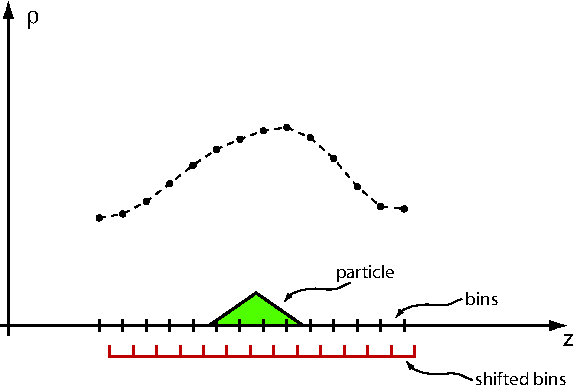
\includegraphics[height=8.4cm]{csr-bin.pdf} \caption[CSR Calculation] {The Coherent
Synchrotron Radiation kick is calculated by dividing longitudinally a bunch into a number of
bins. To smooth the computed densities, each particle of the bunch is considered to have a
triangular density distribution.}  \label{f:csr.bin}
\end{figure}

The electric field $\bfE$ felt by particle $A$ due to particle $B$ can be described using the
Li\'{e}nard-Wiechert formula \cite{b:csr}. The field is singular as the distance between particles
goes to zero so one approach to handling this is to decompose the field into two parts: One part,
called the ``space charge'' (SC) or ``Coulomb'' term, $\bfE_{SC}$ is the field that would result if
the particles where moving without acceleration along a straight line. The ``Coherent Synchrotron
Radiation'' (CSR) term $\bfE_{CSR}$ is everything else $\bfE_{CSR} \equiv \bfE - \bfE_{SC}$.
Generally, the longitudinal component of the SC kick is negligible compared to the CSR kick at large
enough particle energies.

The SC term is singular at small distances while the CSR term is not. This being the case, it is
possible to model the CSR term using a 1-dimensional formalism where the beam is approximated as a
line charge\cite{b:csr,b:csr2}. In this formalism, the CSR kick is strictly longitudinal.

Transport through a lattice element with SC and CSR involves a beam of particles. The lattice
element is divided up into a number of slices. Transport through a slice is a two step process. The
first step is to give all the particles a kick due to SC and CSR. The second step is transport of
all particles from one slice to the next without any interaction between particles. User settable
parameters pertinent to the CSR calculation are listed in \sref{s:sc.com}.

%-----------------------------------------------------------------   
\subsection{1\_Dim CSR Calculation}
\label{s:csr.1d}

When an element's \vn{csr_method} is set to \vn{1_dim} (\sref{s:csr.sc.meth}), The particle-particle
CSR kick is calculated by dividing the bunch longitudinally into a number of bins. To smooth the
computed bin densities, each particle of the bunch is considered to have a triangular density
distribution as shown in \fig{f:csr.bin}.  The particle density of a bin is calculated by summing
the contribution from all the particles. The contribution of a given particle to a given bin is
calculated from the overlap of the particle's triangular density distribution with the bin. For the
CSR kick, the density is actually calculated for a second set of staggered bins that have been
offset by 1/2 the bin width with respect to the first set. This gives the density at the edges of
the original set of bins. The density is considered to vary linearly between the computed density
points. For a description of the parameters that affect the CSR calculation see
Section~\sref{s:sc.com}.

%-----------------------------------------------------------------   
\subsection{Slice Space Charge Calculation}
\label{s:sc.slice}

When an element's \vn{space_charge_method} is set to \vn{slice} (\sref{s:csr.sc.meth}), the
calculation of the SC kick uses, the same particle binning as is used with the \vn{1_dim} CSR
calculation (\sref{s:csr.1d}). The kick is divided into longitudinal and a transverse parts. The
transverse part uses the same Bassetti--Erskine complex error function formula\cite{b:talman} as
with the beam-beam interaction (\sref{s:beambeam.std}) except here, since all the particles are
moving in the same direction, the kicks due to the electric and magnetic fields generated by a given
particle tend to cancel
\begin{align}
  K_y(\text{CS}) + i \, K_x(\text{CS}) &=
  \frac{r_e \, \rho(z)}{\gamma^3 \, e} \cdot
  \sqrt{\frac{2 \, \pi \, (\sigma_x + \sigma_y)}{\sigma_x - \sigma_y}} \label{fsp1r} \\
  & \qquad \left\{ w \left[ \frac{x + i \, y}{\sqrt{2 (\sigma_x^2 - \sigma_y^2)}} \right] -
  \exp \left[ -\frac{x^2}{2 \, \sigma_x^2} - \frac{y^2}{2 \, \sigma_y^2} \right] \cdot
  w \left[ \frac{x \, \frac{\sigma_y}{\sigma_x} + i \, y \, \frac{\sigma_x}{\sigma_y}}
  {\sqrt{2 (\sigma_x^2 - \sigma_y^2)}} \right] \right\}
  \nonumber
\end{align}
where $K(\text{CS})$ is the CS kick per unit length of travel of the beam, $\rho(z)$ is
the density of particles per unit length evaluated at the $z$ position of the kicked
particle, $e$ is the charge on the electron,  and $w$ is the complex error function.

The longitudinal SC kick is given by Eq.~(31) of Sagan\cite{b:csr} 
\begin{equation}
 d K_{\mbox{\tiny SC}} =
  \frac{ r_c m c^2 \, \mbox{sign}(\zeta)\rho(z')dz'}
  {\sigma_x \, \sigma_y \, \exp
  \left[ \frac{x^2}{2 \, \sigma_x^2} + \frac{y^2}{2 \, \sigma_y^2} \right] +
  \frac{\sigma_x^2 + \sigma_y^2}{\sigma_x + \sigma_y} \, \gamma |\zeta| + \gamma^2\zeta^2}\ ,
  \label{kelsz}
\end{equation}
where $\zeta$ is the longitudinal distance between the kick point and the slice doing the kicking.
There are two simulation modes for the longitudinal SC kick. In both these modes, the kick is
evaluated at the center plane of each slice. The kick is a sum kicks from all the slices. Since the
thickness of the slices is, in general, not negligible, the the integral over a slice is used to
calculate the kick. The total kick $K_{\mbox{\tiny SC}}(j)$ at slice $j$ is
\begin{equation}
  K_{\mbox{\tiny SC}} (j) = 
  \sum_i \int_{\zeta_{ij}-dz_s/2}^{\zeta_{ij}+dz_s/2} d\zeta \, dK_{\mbox{\tiny SC}}
\end{equation}
where the sum is over all slices $i$, $\zeta_{ij}$ is the distance between slices $i$ and $j$, and
$dz_s$ is the slice thickness. An analytic expression of the above integral is easily
calculated assuming that the charge density $\rho(z)$ is linearly varying within a given slice.  For
brevity's sake, the calculation is not explicitly presented here. Once the kick at the slice center
planes is calculated, the kick given to a particle is calculated using linear interpolation.

One mode for calculating the transverse SC kick which is computationally fast, ignores the
transverse dependence of the kick and just evaluates the kick on the beam centerline. The other
simulation mode represents the kick due to a given slice using a Pad{\'e} approximant of form
\begin{equation}
  \int_{\zeta_{ij}-dz_s/2}^{\zeta_{ij}+dz_s/2} d\zeta \, dK_{\mbox{\tiny SC}}
  \simeq \frac{1}{a_{00} + a_{20} x^2 + a_{40} x^4 + a_{02} y^2 + a_{04} y^4 + a_{22} x^2 \, y^2}
\end{equation}
the \vn{a_{mn}} are calculated from an analytic formula derived from integrating \Eq{kelsz}. The
reason for using this form is that it is a reasonable approximation even for very large $x$ or $y$
in that the actual and approximate kick both go to zero in this limit. That this Pad{\'e}
approximant is reasonable is dependent upon the fact that all the $a_{mn}$ for a slice are either
all positive or all negative. Kicks from different slices can be combined using standard
Differential Algebra techniques to give a summed kick in the same form as above. To avoid
divergences, for a given $j$ where the kick is evaluated, all the kicks from slices with negative
coefficients are combined together and all the kicks from slices with positive coefficients are
combined together and the total kick is then the sum of the ``positive kick'' part and the
``negative kick'' part. The kick applied to a particle is calculated by first evaluating the kick,
at the particle's $x$ and $y$, at the neighboring slices and then using linear interpolation.

Note: Match elements (\sref{s:match}) can have orbit shifts which are not well handled by the CSR
algorithm. For this reason, match elements are ignored in the CSR calculation.

%-----------------------------------------------------------------   
\subsection{FFT_3D Space Charge Calculation}
\label{s:sc.fft}

When an element's \vn{space_charge_method} is set to \vn{fft_3d} (\sref{s:csr.sc.meth}), the space
charge calculation uses code from the OpenSC package developed by Rob Ryne and Chris Mayes
\cite{b:opensc}. The method works by calculating the field due to the particle on a 3D grid and then
interpolating the field to the points where the particles are. This method will be able to handle
lower energy bunches than the \vn{slice} method (\sref{s:sc.slice}) the disadvantage is that the
\vn{fft_3d} method will be slower. Another point to keep in mind is that the \vn{fft_3d} method
currently ignores image charge forces due to an emitting cathode and so will not be accurate for
tracking at the very lowest energies near the emitter.

Note: The mesh size is set by the \vn{csr_pram} parameter \vn{space_charge_mesh_size}
(\sref{s:sc.com}).

%-----------------------------------------------------------------   
\section{High Energy Space Charge}
\label{s:he.space.charge}
\index{CSR|hyperbf}

\bmad has a code module for simulating the effect of space charge (SC) at high energies. This is
separate from the regular space charge calculation of \sref{s:csr}. Thus it should be noted that
turning on of both the regular space charge and the high energy space charge in the same element
will result in double counting of the space charge effect.

The advantage of the high energy space charge algorithm is that the kick on a given particle is
computed assuming a Gaussian beam with the beam size calculated using emittances supplied by the
user. Thus the high energy space charge calculation can be done in single particle tracking
(\sref{c:multi.sim}) as opposed to the beam tracking that must be used for the regular space charge
calculation. The other advantage is that the high energy space charge calculation is quick since it
is assumed that the kick is small enough so that the kick is only applied once per lattice
element. The disadvantage of the high energy space charge calculation is that there is the
assumption that the beam distribution is Gaussian which is generally acceptable for storage rings at
relatively high energy but will not accurate in other situations.

If a \bmad based program has been constructed to use the high energy space charge module (the
documentation for the program should indicate if this is true), the high energy space charge force
can be turned on or off by setting the \vn{bmad_com[high_energy_space_charge_on]} parameter
(\sref{s:bmad.common}, \sref{s:beginning}). 

The high energy space charge kick is computed assuming a gaussian bunch shape 
\begin{align}
  K_y + i \, K_x &=
  \frac{r_e \, N}{\gamma^3 \, \sigma_z} \, \exp \left[ \frac{z^2}{2 \, \sigma_z} \right] \cdot
  \sqrt{\frac{\sigma_x + \sigma_y}{\sigma_x - \sigma_y}} \label{fsp1r2} \\
  & \qquad \left\{ w \left[ \frac{x + i \, y}{\sqrt{2 (\sigma_x^2 - \sigma_y^2)}} \right] -
  \exp \left[ -\frac{x^2}{2 \, \sigma_x^2} - \frac{y^2}{2 \, \sigma_y^2} \right] \cdot
  w \left[ \frac{x \, \frac{\sigma_y}{\sigma_x} + i \, y \, \frac{\sigma_x}{\sigma_y}}
  {\sqrt{2 (\sigma_x^2 - \sigma_y^2)}} \right] \right\}
  \nonumber 
\end{align}
where $N$ is the number of particles in the bunch. This equation is similar to \Eq{fsp1r} except
that $\rho(z)$ has been replaced assuming that the longitudinal distribution is Gaussian. For
particles close to the bunch core the kick is linear with displacement giving rise to a tune shift
\cite{b:decking}.

The high energy space charge calculation ignores any CSR effects and ignores any longitudinal kicks
and is thus not a good approximation at lower energies. See the discussion in \cite{b:csr} for more
details.






